\documentclass[presentation]{beamer}

\usepackage{tikz}
\usetikzlibrary{positioning,calc}
\usetikzlibrary{shapes.geometric}
\usetikzlibrary{backgrounds}% only to show the bounding box
\usetikzlibrary{shapes,arrows}
\usepackage{pgfplots}
\usepackage{pgfplotstable}
\usetikzlibrary{pgfplots.groupplots}
\pgfplotsset{compat=1.12}
\usepackage{appendixnumberbeamer}
\usepackage{amsmath}
\date{8th June 2016}
\usetheme{metropolis}

\pgfplotscreateplotcyclelist{decent cycle}{%
  {blue, mark=*, mark options={fill=blue},
    mark size=2pt},
  {cyan, mark=square*, mark options={fill=cyan},
    mark size=2pt},
  {magenta, mark=triangle*, mark options={fill=magenta},
    mark size=3pt},
  {blue, mark=*, mark options={fill=blue},
    mark size=2pt},
  {cyan, mark=square*, mark options={fill=cyan},
    mark size=2pt},
  {magenta, mark=triangle*, mark options={fill=magenta},
    mark size=3pt},
}

\pgfplotsset{
  decent/.style={
    cycle list name=decent cycle,
  }
}
\renewcommand{\vec}[1]{\ensuremath{\boldsymbol{#1}}}
\newcommand{\ddt}[1]{\frac{\partial #1}{\partial t}}
\newcommand{\zhat}{\hat{\vec{z}}}
\newcommand{\W}{\ensuremath{\mathbb{W}}}

\DeclareMathOperator{\grad}{grad}
\let\div\relax
\DeclareMathOperator{\div}{div}
\DeclareMathOperator{\curl}{curl}
\newcommand{\vsubset}[1]{\rotatebox[origin=c]{90}{\ensuremath{\subset}}}
\newcommand{\inner}[2]{\ensuremath{\langle #1, #2 \rangle}}
\author{Lawrence Mitchell\inst{1}}
\institute{
\inst{1}Departments of Computing and Mathematics, Imperial College
London
}

\graphicspath{{./\jobname.figures/}}

\newcommand{\arxivlink}[2]{%
  \href{http://www.arxiv.org/abs/#1}%
  {{\small\texttt{arXiv:\,#1\,[#2]}}}%
}
\newcommand{\doilink}[1]{%
  \href{http://dx.doi.org/#1}%
  {{\small\texttt{doi:\,#1}{}}}%
}
\usepackage[url=false,
            doi=true,
            isbn=false,
            style=authoryear,
            firstinits=true,
            uniquename=init,
            backend=biber]{biblatex}

\setbeamertemplate{bibliography item}{}
\renewcommand{\bibfont}{\footnotesize}
\addbibresource{references.bib}

\setlength{\bibitemsep}{1ex}

\renewbibmacro{in:}{}
\DeclareFieldFormat[article]{volume}{\textbf{#1}}
\DeclareFieldFormat{doi}{%
  doi\addcolon%
  {\scriptsize\ifhyperref{\href{http://dx.doi.org/#1}{\nolinkurl{#1}}}
    {\nolinkurl{#1}}}}
\AtEveryBibitem{%
\clearfield{pages}%
\clearfield{issue}%
\clearfield{number}%
}

\usepackage{minted}

\title{Firedrake: automating the finite element method by composing
  abstractions}

\begin{document}
\maketitle

\section{Introduction}

\begin{frame}
  \frametitle{Firedrake development team}
  \begin{itemize}
  \item[IC] David A.~Ham, Mikl\'os Homolya, Fabio Luporini, Gheorghe-Teodor
    Bercea, Paul H.~J.~Kelly
  \item[Bath] Andrew T.~T.~McRae
  \item[ECMWF] Florian Rathgeber
  \end{itemize}
  \begin{center}
    \url{www.firedrakeproject.org}
  \end{center}
\end{frame}

\begin{frame}[fragile]
  \frametitle{How do \emph{you} solve the Poisson equation?}
  \begin{columns}
    \begin{column}{0.65\textwidth}
\begin{minted}[fontsize=\tiny]{python}
from firedrake import *
mesh = UnitSquareMesh(100, 100)
V = FunctionSpace(mesh, "RT", 2)
Q = FunctionSpace(mesh, "DG", 1)
W = V*Q
u, p = TrialFunctions(W)
v, q = TestFunctions(W)

a = dot(u, v)*dx + div(v)*p*dx + div(u)*q*dx
L = -Constant(1)*v*dx
u = Function(W)
solve(a == L, u, solver_parameters={
    "ksp_type": "gmres", 
    "ksp_rtol": 1e-8,
    "pc_type": "fieldsplit",
    "pc_fieldsplit_type": "schur",
    "pc_fieldsplit_schur_fact_type": "full",
    "pc_fieldsplit_schur_precondition": "selfp",
    "fieldsplit_0_ksp_type": "preonly",
    "fieldsplit_0_pc_type": "ilu",
    "fieldsplit_1_ksp_type": "preonly",
    "fieldsplit_1_pc_type": "hypre"
})
\end{minted}
    \end{column}
    \hspace{-4em}
    \begin{column}{0.5\textwidth}
      Find $u\in V\times Q\subset H(\div)\times L^2$ s.t.
      \begin{align*}
        \inner{u}{v} + \inner{\div v}{p} &= 0 \quad\forall\, v \in V\\
        \inner{\div u}{q} &= -\inner{1}{q}\quad\forall\, q \in Q.
      \end{align*}
    \end{column}
  \end{columns}
\end{frame}


\begin{frame}
  How do we develop models?

  \begin{itemize}
  \item Choose equations
  \item Pick method/discretisation
  \item Decide on implementation language, target architecture
  \item Write code to implement method
  \end{itemize}
\end{frame}

\begin{frame}[fragile]
  \frametitle{FEM pseudocode}

  \begin{onlyenv}<1>
\begin{minted}[fontsize=\tiny]{python}
# x the input fields (e.g. current guess)
def form_residual(x):
    x_l <- x # global to ghosted
    for each element in mesh:
        x_e <- x_l[element] # gather through element map
        for each qp in element:
            basis_fns <- eval_basis_funs(qp)
            J <- compute_geometry(element, qp)
            f_qp <- user_evaluation(qp, basis_fns, x_e)
            # insert into element residual
            f_e <- transform_to_physical(f_qp, J)
        f_l <- f_e # scatter through element map
    f <- f_l # ghosted to global
\end{minted}
  \end{onlyenv}

  \begin{onlyenv}<2>
\begin{minted}[fontsize=\tiny]{python}
            f_qp <- user_evaluation(qp, basis_fns, x_e)
\end{minted}
    \begin{itemize}
    \item Problem-specific variability in \emph{innermost} loop
    \item Efficient implementation may need to:
      \begin{itemize}
      \item vectorize across elements,
      \item vectorize within an element,
      \item exchange loop order,
      \item hoist loop-invariant code,
      \item exploit structure in basis functions.
      \item Choices \emph{will} almost certainly be architecture-dependent.
      \end{itemize}
    \end{itemize}
  \end{onlyenv}
\end{frame}

\begin{frame}[standout]
  Say \emph{what}, not \emph{how}.
\end{frame}

\begin{frame}
  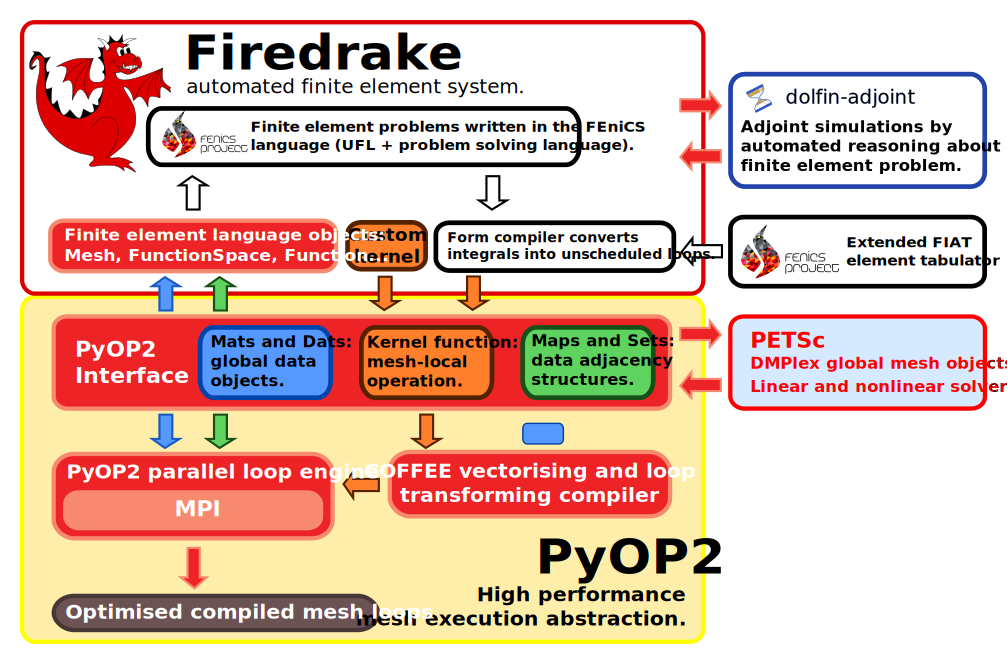
\includegraphics[width=\textwidth]{firedrake-stack}
\end{frame}

\section{Local kernels}

\begin{frame}
  \frametitle{FE compiler}
  Symbolic UFL expression defines \emph{local} (element-wise)
  operation.

  Compilation to executable code is a three-stage process.
  \begin{enumerate}
  \item Remove FE-specific parts in symbolic expression (insert basis
    function evaluation...)
  \item Build loop nest from tensor-algebra expressions
  \item Optimise resulting loop nest and spit out C/intrinsics
  \end{enumerate}
  \begin{center}
    \url{github.com/firedrakeproject/tsfc}
  \end{center}
\end{frame}

\begin{frame}[fragile]
  \frametitle{COFFEE}
  
  No single optimal scheduling of loop nests that occur in finite
  element integration.  Depends on degree, form complexity, basis
  function structure.

  By generating code and passing to a special-purpose optimising
  compiler, we are able to achieve significant reductions in operation
  counts.  Mostly through judicious use of loop-invariant code motion
  and CSE.

%   empirical:
  
% \begin{minted}[fontsize=\tiny]{python}
% for i in ...:
%    for j in ...:
%       for k in ...:
%           A[j, k] += f(i, k)*g(i, j) + ...
% \end{minted}

% General purpose compilers will hoist \verb~g(i, j)~, but not \verb~f(i, k)~.
  \begin{center}
    \url{github.com/coneoproject/COFFEE}\\
    \cite{Luporini:2015} \doilink{10.1145/2687415}
    \cite{Luporini:2016} \arxivlink{1604.05872}{cs.MS}\\
  \end{center}
\end{frame}
\section{Global iteration}

\begin{frame}[fragile]
  \frametitle{PyOP2}
  A library for expressing data parallel iterations
\begin{description}
\item[{\emph{Sets}}] iterable entities
\item[{\emph{Dats}}] abstract managed arrays (data defined on a set)
\item[{\emph{Maps}}] relationships between elements of sets
\item[{\emph{Kernels}}] the "local" computation
\item[{\emph{par\_loop}}] Data parallel iteration over a set
\end{description}
Arguments to parallel loop indicate how to gather/scatter global
data using \emph{access descriptors}

\begin{minted}[fontsize=\tiny]{python}
par\_loop(kernel, iterset, data1(map1, READ), data2(map2, WRITE))
\end{minted}
\begin{center}
  \url{github.com/OP2/PyOP2}\\
  \cite{Rathgeber:2012} \doilink{10.1109/SC.Companion.2012.134}
\end{center}
\end{frame}

\begin{frame}
  \frametitle{Optimising mesh iteration}
  We all know we \emph{ought} to do loop tiling
  \begin{itemize}
  \item Better data reuse/locality
  \item Can hide communication latency
  \end{itemize}
  But it's very invasive to an application (especially an unstructured
  one).

  PyOP2 approach makes it possible to provide loop tiling in a
  semi-automated way within the library.

  Application code does ``whatever'', PyOP2 sees a sequence of
  parallel loops with data dependencies.  Can tile over multiple
  loops.
\end{frame}


\section{Symbolic computation}

\begin{frame}
  \frametitle{Maintaining symbolic information}
  Firedrake uses UFL \cite{Alnaes:2014} to specify problems

  Can perform AD at a high level, resulting in efficient code for
  adjoints, etc...

  Can produce matrix-free with low-order preconditioners
  ``automatically''.  Symbolic reasoning and composition of solvers,
  rather than just algebraic manipulation (all that is available with
  assembled matrices).
  Allows symbolically, rather than just algebraically, expressing
  complex solvers (WIP, with Rob Kirby (Baylor)).
\end{frame}



\begin{frame}
  \frametitle{Mesh iteration}
  Mesh-based solvers execute \emph{local} operation over mesh
  gathering data with some \emph{stencil}.

  PyOP2 captures these iterations and manages the execution.

  Most naive implementation just does ``the iteration you would have
  written''.

  But, we can do more.  In particular, unstructured mesh loop-tiling.
\end{frame}

\begin{frame}
  \frametitle{Solvers}
  
\end{frame}

\begin{frame}
  \frametitle{Applications of Firedrake}
  \begin{itemize}
  \item Colin Cotter (Imperial College).  3D mimetic finite element
    dynamical core for NWP
  \item Onno Bokhove (University of Leeds). Freak waves,
    fluid-structure interactions (boats in waves).
  \item Justin Chang (University of Houston).  Positivity preserving
    methods for advection-diffusion-reaction geochemical systems
  \item Tuomas K\"arn\"a (Oregon Health and Science). 3D coastal and
    estuarine ocean modelling
  \item Andrew McRae, Chris Budd (University of Bath).  $r-$adaptivity
    on the sphere.
  \item Francis Poulin (University of Waterloo).  Stability of jets
    and vortices in the ocean.
  \end{itemize}
\end{frame}
\appendix
\begin{frame}[allowframebreaks]
  \frametitle{References}
  \printbibliography[heading=none]
\end{frame}
\end{document}
